\chapter{Analysephase}

\section{Expected Goals}
\label{goals}
Dieser Abschnitt soll dem Leser den aktuellen Forschungsstand der \textit{Expected Goals} vermitteln, deren Bedeutsamkeit für den Fußballsport dabei explizit aufzeigen, sowie den Einfluss von Data-Mining-Methoden hinsichtlich der Wissensgewinnung darstellen.

\begin{quote}
\textit{\glqq Expected Goals - Das angesagteste Statistikmodell im Profifußball\grqq}
\end{quote}

So betitelt Nils Nordmann seinen Online-Artikel im Interview mit Dustin Böttger, Geschäftsführer von \gls{gsn}, einem der gefragtesten Datenanalysten aus Deutschland, der mit mehreren Bundesligavereinen in Kooperation steht.\seFootcite{}{}{NilsNordmann.2016} Statistische Analysen sind im Bereich des Fußballs keine Neuheit mehr, jedoch liegt der Ursprung der sportlichen Datenanalyse in einer anderen Sportart. Der amerikanische Historiker und Statistiker Bill James veröffentlichte 1977 erste Analysen zwischen geschlagenen und gefangenen Bällen im Baseball, um eine objektive Bewertung der Gesamtleistung eines Spielers aufstellen zu können. Schumaker, Solieman und Chen bezeichnen diese Entwicklung als eine Art \glqq Revolution\grqq-- einen Wandel von traditionellen Statistiken hin zum Wissensmanagement.\seFootcite{Vgl.}{S.36}{Schumaker.2010} Diese löste eine Welle der Erstellung neuer Maßzahlen aus, wovon einige im Jahr 2002 von der amerikanischen Baseball Profimannschaft \textit{Oakland A’s Billy Bean} als Grundlage zur Zusammenstellung eines neuen Teams dienten. Die \textit{Boston Red Sox} ließen sich von dieser Idee inspirieren und  gewannen anschließend sogar 2004 und 2007 die Meisterschaft.\seFootcite{Vgl.}{S.36}{Schumaker.2010} Auch aus anderen Sportarten gibt es vergleichbare Beispiele, wie die digitale Revolution im Basketball im Jahr 1980 durch den Statistiker Dean Oliver, der neue Messwerte zur Beurteilung von Spielern veröffentlichte.\footnote{Dean Oliver beriet 2005 die \textit{Seatlle Supersonics} und verhalf zur amerikanischen Meisterschaft}

Waren im Fußball in der Vergangenheit noch rein quantitative \glspl{kpi} wie der Ballbesitz, die Passquote oder die Anzahl der Torschüsse von Bedeutung, wird das Spiel heutzutage bis in das kleinste Detail (z.B. die Anzahl der vertikal \glqq überspielten\grqq~Gegenspieler durch einen Pass) analysiert. Durch den Fortschritt der Videotechnik können alle Aktionen eines Spieles aufgezeichnet werden, wodurch sich neue stichhaltige Bewertungsmethoden herauskristallisiert haben. Sumpter, Anderson und weitere Fachexperten untersuchen mit Hilfe von Mathematik und Statistik das Spiel und stellen in ihren Ausführungen einige Thesen und Modelle auf.\seFootcite{Vgl.}{}{Sumpter.2016}\seFootcite{Vgl.}{}{Anderson.2014}\seFootcite{Vgl.}{}{Heuer.2010} Eines der momentan angesagten Modelle ist das der \glqq \textbf{Expected Goals}\grqq (\textit{dt. die zu erwartenden Tore}), welches die Qualität von Torschüssen vielseitig, objektiv und plausibel misst.\seFootcite{}{}{NilsNordmann.2016} Dazu wird jedem Schuss, unter der Berücksichtigung von Parametern (wie beispielsweise der Position oder des Körperteils mit dem geschossen wurde), eine bestimmte Erfolgswahrscheinlichkeit zugewiesen. Die Bestimmung der Wahrscheinlichkeit, die Auswahl der einbezogenen Schüsse wie auch Parameter und teilweise das gesamte Modell wird öffentlich von den Analytikern (meist aus Unternehmen der Sportanalyse/-beratung) nur kurz ausgeführt oder gar komplett geheimgehalten. Einblicke in ihre Modellierungen bieten unter anderem Opta Sports\seFootcite{Vgl.}{}{PhilippObloch.2015}, der TV-Sender Sky Sports,\seFootcite{Vgl.}{}{PhilippErtl.2016} oder Experten, wie Michael Caley, in ihren Internetpublikationen.\seFootcite{Vgl.}{}{MichaelCaley.2017} Ein \textit{Expected-Goal-Modell} offeriert eine statistisch belegte und damit objektive Bewertung von Schüssen und bildet einen neuen \gls{kpi} bezüglich der Qualität einer Torchance. Anhand dieser Grundlage ist es möglich, weitere Bewertungsmethoden für Spieler und Mannschaften zu ermitteln, die vor allem im Scouting-Bereich ihre Anwendung finden. Durch die qualitative Bewertung der Schüsse eines Stürmers mittels des Expected-Goal-Modells, kann eine objektive Aussage über dessen Erfolgsquote getroffen werden (beispielsweise ob diese über den erwarteten Toren liegt), welche dann zur Spielersuche herangezogen werden kann. Eine Gefahr in der Modellierung der Expected Goals stellt die \textit{Überparametrisierung} (vgl. \vref{bhm}) dar. Werden zu viele Parameter, z.B. welcher Spieler geschossen hat und ob mit seinem starken oder schwachen Fuß geschossen wurde, seine Tagesform, die Leistung des generischen Torhüters, usw. bei der Modellierung herangezogen, verliert das Modell durch zu viele Details seine Abstraktion und folglich seine allgemeine Aussagekraft (für alle Schüsse). Die Kunst liegt in der \vref{bhm} beschriebenen Balance von \textit{Underfitting} und \textit{Overfitting} des Modells.

Durch die Technisierung der Datenaufnahme im Fußball werden stetig mehr Daten während eines Spieles erhoben\footnote{beispielsweise durch Videobildverarbeitung oder Sensordaten.}, woraus im Laufe einer Saison eine Datenmenge resultiert, die die Leistungsfähigkeit herkömmlicher Analysewerkzeuge übersteigt. Um wertvolle Informationen aus den umfangreich Daten zu extrahieren, greifen auch Datenanalysten im Bereich des Fußball auf die Prozesse und Methoden des Data Minings zurück. Ausführliche Einblicke in die Komplexität der Datenanalyse im Sport stellen unter anderem Schumaker et al. in ihrer Ausarbeitung vor.\seFootcite{Vgl.}{}{Schumaker.2010} Data-Mining-Methode, wie das Clustering zur Einteilung von Spielertypen, die Regressionanalyse zur Ermittlung von Erfolgsfaktoren einer Saison, Entscheidungsbäume zur Bestimmung des perfekten Ein- und Auswechslungszeitpunktes, als auch Neuronale Netze zur Prognose von Spielausgängen, werden hierbei zur Wissensgewinnung verwendet.\seFootcite{Vgl.}{}{GunjanKumar.2013} Darüber hinaus werden einige dieser Techniken zur komplexen Erkennung von Taktiken und Spielphilosophien eingesetzt, welche in der Ausführung von Rein konkretisiert werden.\seFootcite{Vgl.}{}{Rein.2016}




\section{Opta-Spieldaten}
test\seFootcite{Vgl.}{S.1}{OptaSports.2017a}
test\seFootcite{Vgl.}{S.1}{OptaSports.2017b}

\section{Wirtschaftliche Betrachtung}
\label{wa}
In diesem Abschnitt werden die wirtschaftlichen Konsequenzen des Modelles sowohl aus Sicht des Unternehmens, wie auch aus Sicht des Fußballvereines betrachtet.\enlargethispage{2\baselineskip}  Aufgrund von vertraulichen Daten wir die Beispielkalkulation auf Basis fiktiver Daten durchgeführt.

\paragraph{Sichtweise des Unternehmens}

\begin{figure}[H]
\centering
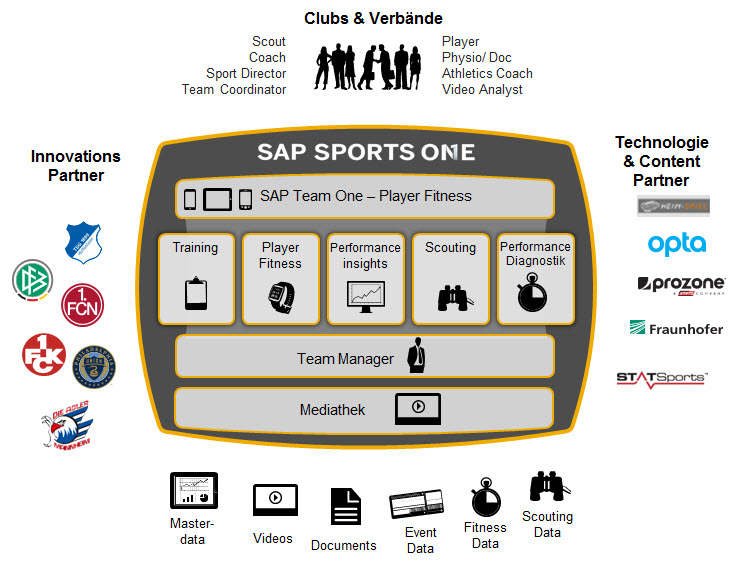
\includegraphics[scale=0.575]{se-wa-jpg/sportsone}
\caption{Überblick über Sports One}
\label{sportsone}
\end{figure}

Sports One ist eine von SAP speziell für die Sportbranche entwickelte Software-Lösung und bietet derzeit Funktionen in den Bereichen Team Management, Spiel- und Trainingsanalysen, Spielerfitness, Leistungsdiagnostik und Scouting an, welche im Gesamtkontext des Produktes in \vref{sportsone} dargestellt sind. Nach der Modellierung der Funktion stellt sich aus Sicht der SAP die Frage, ob eine Investition in die Erstellung einer darauf aufbauenden Software rentabel ist. Die folgende (durchschnittliche) Amortisationsrechnung soll darüber Aufschluss geben, wobei aufgrund der Schnelllebigkeit der Softwarebranche diesbezüglich mit einer Amortisationszeit von drei Jahren gerechnet wird. Die Entwicklung des grundlegenden mathematischen Modelles nahm in etwa 50 Werktage und die Kapazität eines Mitarbeiters in Anspruch. Bei einem fiktiven internen Tagessatz von \textsf{1.500\,\euro} ergeben sich dadurch Kosten in Höhe von \textsf{75.000\,\euro}. Durch die Verwendung der Testversion von MATLAB für Studenten fielen die normalerweise anfallenden Lizenzkosten weg. Weiterhin wurden die für das Modell zugrundeliegenden Daten von Opta Sports zu Forschungszwecken kostenfrei bereitgestellt, sodass letztlich auch keine Kosten für den Einkauf der Daten aus Sicht des Unternehmens entstanden. Für die Entwicklung dieses zusätzlichen Software-Features für den Kunden entstehen unterschiedliche Kosten, die nachfolgend exemplarisch aufgelistet werden (vgl. \vref{calc}). Ein Team aus drei vollbeschäftigten Mitarbeiter mit einem internen Tagessatz von \textsf{1.500\,\euro} würde für eine solche Umsetzung schätzungsweise drei Monate benötigen. Diese Phasen lässt sich dabei in die Konzepterstellung (Anteil 30\%), die Architekturplanung (30\%), die Implementierung und Integration in den Scoutingbereich von Sports One (20\%), die Validierung (15\%) sowie die Dokumentation (5\%) der Software untergliedern, wodurch \textsf{315.000\,\euro} in Summe für Personalkosten entstehen. Zusätzlich entstehen weitere Einzelkosten durch die kommerzielle Nutzung von MATLAB in Höhe von \textsf{1.000\,\euro} monatlich. Die Gemeinkosten für die Erstellung der Software umfassen Kosten der Raumnutzung, Abschreibungen technischer Geräte, sowie Energiekosten in Höhe von insgesamt \textsf{4.000\,\euro}. Daraus ergeben sich zusammenfassend Investitionskosten von \textsf{397.000\,\euro}. Nach der Auslieferung der fertigen Software fallen laufende Ausgaben, die beispielsweise die Lizenz-, Wartungs- und Supportkosten, aber auch Vertriebskosten für die Propagierung des Features enthalten, an. Um auch in der Zukunft wettbewerbsfähig bleiben zu können, werden sowohl das Modell als auch die Software stetig erweitert und verbessert, wodurch in Summe \textsf{350.000\,\euro} an laufenden jährlichen Ausgaben entstehen. Aufgrund der Vertraulichkeit können die jährlichen Lizenzkosten der Nutzung und der Wartung des gesamten Sport One Produktes nicht genannt werden. Aus diesem Grund wird eine Rückwärtsrichtung angewandt, um die benötigten jährlichen Einnahmen zu ermitteln, welche die Investition innerhalb der angestrebten drei Jahren amortisieren sollen. Diese belaufen sich insgesamt auf rund \textsf{480.000\,\euro} und bilden dabei einen Gewinnaufschlag von \textsf{38\,\%} bezogen auf die laufenden Ausgaben. Diese Marge liegt in der üblichen Größenordnung der SAP. \vref{calc} fasst die Berechnungen in einem übersichtlichen Schaubild zusammen.

\begin{sidewaystable}
\centering
\caption{Amortisationsrechnung}
\label{calc}
\begin{tabular}{llrlllrlll}
\cline{1-3} \cline{5-7}
\multicolumn{1}{|l}{\textbf{}}             & \multicolumn{1}{c}{\textbf{Investition}}        & \multicolumn{1}{l|}{}                            & \multicolumn{1}{l|}{} & \multicolumn{3}{c|}{\textbf{Laufende jährliche Ausgaben}}                                                                  &  &  &  \\ \cline{1-3} \cline{5-7}
\multicolumn{2}{|c|}{{\ul Modell}}                                                           & \multicolumn{1}{l|}{}                            & \multicolumn{1}{l|}{} & \textit{Lizenzkst.}      & \multicolumn{1}{l|}{}                        & \multicolumn{1}{r|}{12.000,00 \euro}                 &  &  &  \\
\multicolumn{1}{|l}{\textit{Personalkst.}} & \multicolumn{1}{l|}{}                           & \multicolumn{1}{r|}{75.000,00\euro}                  & \multicolumn{1}{l|}{} & \textit{Wartungkst.}     & \multicolumn{1}{l|}{}                        & \multicolumn{1}{r|}{40.000,00 \euro}                 &  &  &  \\
\multicolumn{1}{|l}{\textit{Lizenzkst.}}   & \multicolumn{1}{l|}{}                           & \multicolumn{1}{r|}{0,00\euro}                       & \multicolumn{1}{l|}{} & \textit{Supportkst.}     & \multicolumn{1}{l|}{}                        & \multicolumn{1}{r|}{60.000,00 \euro}                 &  &  &  \\
\multicolumn{1}{|l}{}                      & \multicolumn{1}{r|}{$\sum$}                          & \multicolumn{1}{r|}{{\ul \textbf{75.000,00 \euro}}}  & \multicolumn{1}{l|}{} & \textit{Erweiterungkst.} & \multicolumn{1}{l|}{}                        & \multicolumn{1}{r|}{150.000,00 \euro}                &  &  &  \\ \cline{1-3}
\multicolumn{2}{|c|}{{\ul Software}}                                                         & \multicolumn{1}{l|}{}                            & \multicolumn{1}{l|}{} & \textit{Beratungkst.}    & \multicolumn{1}{l|}{}                        & \multicolumn{1}{r|}{30.000,00 \euro}                 &  &  &  \\
\multicolumn{1}{|l}{\textit{Personalkst.}} & \multicolumn{1}{l|}{}                           & \multicolumn{1}{l|}{}                            & \multicolumn{1}{l|}{} & \textit{Vertriebkst.}    & \multicolumn{1}{l|}{}                        & \multicolumn{1}{r|}{50.000,00 \euro}                 &  &  &  \\
\multicolumn{1}{|l}{}                      & \multicolumn{1}{l|}{\textit{Konzepterstellung}} & \multicolumn{1}{r|}{63.000,00 \euro}                 & \multicolumn{1}{l|}{} & \textit{Verwaltungkst.}  & \multicolumn{1}{l|}{}                        & \multicolumn{1}{r|}{8.000,00 \euro}                  &  &  &  \\ \cline{5-7}
\multicolumn{1}{|l}{}                      & \multicolumn{1}{l|}{\textit{Architketur}}       & \multicolumn{1}{r|}{63.000,00 \euro}                 & \multicolumn{1}{l|}{} &                          & \multicolumn{1}{r|}{\textbf{Gesamtausgaben}} & \multicolumn{1}{r|}{{\ul \textbf{350.000,00 \euro}}} &  &  &  \\ \cline{5-7}
\multicolumn{1}{|l}{}                      & \multicolumn{1}{l|}{\textit{Implementierung}}   & \multicolumn{1}{r|}{42.000,00 \euro}                 &                       &                          &                                              & \multicolumn{1}{l}{}                             &  &  &  \\ \cline{5-7}
\multicolumn{1}{|l}{}                      & \multicolumn{1}{l|}{\textit{Validierung}}       & \multicolumn{1}{r|}{31.500,00 \euro}                 & \multicolumn{1}{l|}{} & \multicolumn{3}{c|}{\textbf{Berechnung der benötigten Einnahmen}}                                                          &  &  &  \\ \cline{5-7}
\multicolumn{1}{|l}{}                      & \multicolumn{1}{l|}{\textit{Dokumentation}}     & \multicolumn{1}{r|}{10.500,00 \euro}                 & \multicolumn{1}{l|}{} & Amortisationszeit        & \multicolumn{1}{r}{}                         & \multicolumn{1}{r|}{3 Jahre}                     &  &  &  \\
\multicolumn{1}{|l}{}                      & \multicolumn{1}{r|}{\textit{$\sum$}}                 & \multicolumn{1}{r|}{\textbf{210.000,00 \euro}}       & \multicolumn{1}{l|}{} & Formel                   & \multicolumn{2}{r|}{$AZ = \frac{Investition}{Einnahmen-Ausgaben}$}                                                                          &  &  &  \\
\multicolumn{1}{|l}{}                      & \multicolumn{1}{l|}{\textit{Nebenkosten (SV)}}       & \multicolumn{1}{r|}{105.000,00 \euro}                & \multicolumn{1}{l|}{} & Umstellung               & \multicolumn{2}{r|}{$Einnahmen = (\frac{Investition}{AZ} + Ausgaben)$}                                                                          &  &  &  \\
\multicolumn{1}{|l}{}                      & \multicolumn{1}{r|}{$\sum$}                          & \multicolumn{1}{r|}{\textbf{315.000,00 \euro}}       & \multicolumn{1}{l|}{} & \textbf{Einnahmen}       & \multicolumn{1}{r}{\textbf{}}                & \multicolumn{1}{r|}{\textbf{482.333,33 \euro}}       &  &  &  \\
\multicolumn{1}{|l}{Lizenzkst.}            & \multicolumn{1}{l|}{}                           & \multicolumn{1}{r|}{3.000,00 \euro}                  & \multicolumn{1}{l|}{} & \textit{Gewinnzuschlag}  & \multicolumn{1}{r}{\textit{}}                & \multicolumn{1}{r|}{\textit{38\%}}               &  &  &  \\ \cline{5-7}
\multicolumn{1}{|l}{Raumkst.}              & \multicolumn{1}{l|}{}                           & \multicolumn{1}{r|}{3.000,00 \euro}                  &                       &                          &                                              & \multicolumn{1}{l}{}                             &  &  &  \\
\multicolumn{1}{|l}{Abschreibungen}        & \multicolumn{1}{l|}{}                           & \multicolumn{1}{r|}{500,00 \euro}                    &                       &                          &                                              & \multicolumn{1}{l}{}                             &  &  &  \\
\multicolumn{1}{|l}{Energiekst.}           & \multicolumn{1}{l|}{}                           & \multicolumn{1}{r|}{500,00 \euro}                    &                       &                          &                                              & \multicolumn{1}{l}{}                             &  &  &  \\ \cline{1-3}
\multicolumn{1}{|l}{}                      & \multicolumn{1}{r|}{\textbf{Gesamtkosten}}      & \multicolumn{1}{r|}{{\ul \textbf{397.000,00 \euro}}} &                       &                          &                                              & \multicolumn{1}{l}{}                             &  &  &  \\ \cline{1-3}
                                           &                                                 & \multicolumn{1}{l}{}                             &                       &                          &                                              & \multicolumn{1}{l}{}                             &  &  & 
\end{tabular}
\end{sidewaystable} 


\paragraph{Sichtweise des Vereins}
Mit Hilfe einer solcher integrierten Anwendung im Scoutingbereich ergeben sich aus der Sicht eines Fußballvereines einige wirtschaftliche Implikationen. Neben den Lizenzkosten des Sport One Produktes müssen auch Spieldaten über einen Datenprovider, wie zum Beispiel Opta Sports, eingekauft werden, wodurch sich zunächst Ausgaben ergeben. Durch die Nutzung des Features der \textit{Expected Goals} und der dadurch resultierenden objektiven Bewertung eines Spielers, können im Gegenzug einige Kosten eingespart werden. Beispielsweise werden für die Suche nach einem neuen Mittelstürmer einige Scouts beauftragt, die einerseits dafür bezahlt werden müssen, andererseits durch die Fahrten auf die entsprechenden Spiele auch weitere Kosten verursachen. Durch die Vorselektion der Spieler anhand dieser neuen KPI wird die Auswahl der zur relevanten Spieler deutlich reduziert und somit folglich auch die Anzahl der benötigten Scouts. Letztlich muss ein Spieler immer vor seiner Verpflichtung subjektiv eingeschätzt werden, da dieser auch beispielsweise von der Persönlichkeit in die Teamstruktur passen muss. Die kann durch objektive Kennzahlen nicht gemessen werden. Des Weiteren können durch die Verwendung dieses Scoutingfeatures verborgene Talente entdeckt werden, die in einem frühen Stadium noch zu einem geringen Preis verpflichtet werden und einige Jahre später durch einen Verkauf an einen internationalen Top-Verein Millionen einbringen können, wodurch sich die Investition in diese Software-Lösung ausreichend gelohnt hätte. Wie in den genannten Beispielen aus dem Bereich des Baseballs und des Basketballs (vgl. \vref{goals}) ist es im Fußball nicht möglich eine ganze Mannschaft, bestehend aus elf Spielern, anhand dieser einzelnen Kennzahl vollständig zusammenzustellen, da in einem solchen Mannschaftssport weitere Faktoren, wie z.B. taktisches Verständnis oder Teamfähigkeit, eine wichtige Rolle einnehmen. 